\documentclass[tikz,border=12pt]{standalone}
\usepackage{fontspec}
\setmainfont{Segoe UI}
\usepackage{amsmath,amssymb}
\usepackage{tikz}

\usetikzlibrary{calc,arrows.meta}

\begin{document}
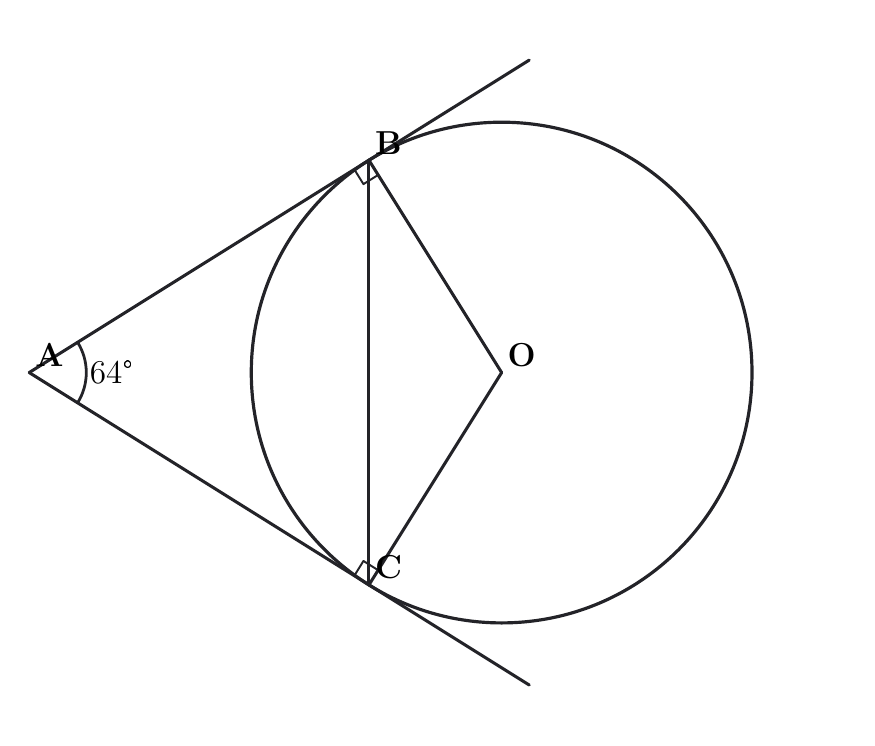
\begin{tikzpicture}[x=1.0000cm,y=1cm,line cap=round,line join=round]
\definecolor{linec0}{RGB}{35,35,40}
\definecolor{linec1}{RGB}{35,35,40}
\definecolor{linec2}{RGB}{35,35,40}
\definecolor{linec3}{RGB}{35,35,40}
\definecolor{linec4}{RGB}{35,35,40}
\definecolor{linec5}{RGB}{35,35,40}
\definecolor{edgecol}{RGB}{35,35,40}
\definecolor{hicol}{RGB}{35,35,40}
\definecolor{angcol}{RGB}{35,35,40}
\coordinate (A) at (0.0000,0.0000);
\coordinate (P) at (6.3504,3.9682);
\coordinate (Q) at (6.3504,-3.9682);
\coordinate (B) at (4.3151,2.6964);
\coordinate (C) at (4.3151,-2.6964);
\coordinate (O) at (6.0000,0.0000);
\draw[edgecol,line width=1.1pt] (A) -- (P);
\draw[edgecol,line width=1.1pt] (A) -- (Q);
\draw[edgecol,line width=1.1pt] (O) -- (B);
\draw[edgecol,line width=1.1pt] (O) -- (C);
\draw[edgecol,line width=1.1pt] (B) -- (C);
\draw[edgecol,line width=1.15pt] (O) circle [x radius=3.1795, y radius=3.1795];
\path (1.621,-4.380) rectangle (10.380,4.380);
\draw[edgecol,line width=0.7pt] (4.129,2.580) -- (4.245,2.393) -- (4.432,2.510);
\draw[edgecol,line width=0.7pt] (4.129,-2.580) -- (4.245,-2.393) -- (4.432,-2.510);
\draw[edgecol,line width=1.00pt] (0.000,0.000)++(32.00:0.725) arc[start angle=32.00, delta angle=-64.00, radius=0.725];
\node[text=black,font=\large] at (1.045,0.000) {64°};
\node[font=\bfseries\large,inner sep=2pt,anchor=south west] at (0.000,0.000) {A};
\node[font=\bfseries\large,inner sep=2pt,anchor=south west] at (4.315,2.696) {B};
\node[font=\bfseries\large,inner sep=2pt,anchor=south west] at (4.315,-2.696) {C};
\node[font=\bfseries\large,inner sep=2pt,anchor=south west] at (6.000,0.000) {O};
\end{tikzpicture}
\end{document}
